\section{Appendix}

\subsection{Large Amplitude Elongated-Body Theory}
\label{sec:large_amplitude_ebt}
The thrust of a fish swimming in an inviscid fluid can be described by Lighthill's Elongated-body theory (EBT)~\cite{lighthill1971large}. To calculate the thrust predicted by EBT, we make use of a simplified version of the reaction force expression from Lighthill~\cite{lighthill1971large}, which uses significantly different notation,
\begin{equation}
    f_\textrm{EBT} \approx \frac{1}{2}m\dot{x}^2,
\end{equation}
where we have evaluated the expression for the marker closest to the tail and we have assumed the unit vectors $\frac{\partial x}{\partial a}\approx 0$ and $\frac{\partial y}{\partial a} \approx 1$ when considering small tail deformations in dynamic actuation. Note that $\dot{x}$ is velocity tangential to the fin chord.

We also use Lighthill's expression for the virtual mass $m=\frac{1}{4} \pi \rho s^2$, where $\rho$ is the density of the fluid and $s$ is the cross-sectional depth, by estimating the geometry from the CAD model of our robotic fish.




% \iffalse
\subsection{Load Cell Measurement Dynamics}
\label{sec:load_cell_measurement}

We choose to model the dynamics of the load cell measurement jig (\Cref{fig:experimental_setup}) as a lumped element system shown in \Cref{fig:load_cell_dynamics}. We assume that the stiffness of the fixture is far greater than the stiffness of the connection between the load cell and the fish. 
Solving for the transfer function describing the load cell dynamics, we have
\begin{equation}
    \frac{f_\textrm{m}}{f_\textrm{hydro}} = \frac{bs+k}{ms^2+bs+k},
    \label{eqn:measurement_dynamics}
\end{equation}
where $s$ is the complex Laplace variable. From this model, it is clear how the measured force $f_\textrm{m}$ can be negative even for strictly positive $f_\textrm{hydro}$ as discussed in \Cref{sec:learned_hydrodynamics}. 

It is possible to measure each parameter in \Cref{eqn:measurement_dynamics} and compensate it by inverting the transfer function, however, our proposed data-driven neural network force predictor is agnostic to the dynamics of the measurement system.

\begin{figure}[htb]
    \centering
    \begin{circuitikz}
    
    %ground
    \pattern[pattern=north east lines] (0,0) rectangle (.25,3);
    \draw[thick] (.25,0) -- (.25,3);
    
    \draw (.25,1) to[spring, l_=$k$] (2,1);
    \draw (.25,2) to[damper, l=$b$] (2,2);
    \draw[fill=gray!40] (2,0.5) rectangle (4,2.5);
    \node at (3,1.5) {$m$};
    
    \draw[thick, ->] (5,1.5) -- (4,1.5);
    \node at (4.5,2) {$f_\textrm{hydro}$};
    
    \draw[thick, ->] (0,1.5) -- (-1,1.5);
    \node at (-0.5,2) {$f_\textrm{m}$};
    
    \end{circuitikz}
    \caption{Load cell dynamics. The force $f_\textrm{m}$ is measured with a pre-calibrated load cell. The force $f_\textrm{hydro}$ is the actual hydrodynamic force experienced by the fish. The stiffness $k$ and the damping coefficient $b$ describe the lumped mechanical impedance of the measurement system. The lumped mass $m$ is dominated by the fish. The wall is the connection point to the load cell.}
    \label{fig:load_cell_dynamics}
\end{figure}
% \fi

\iffalse
\begin{figure}[htb]
    \centering
    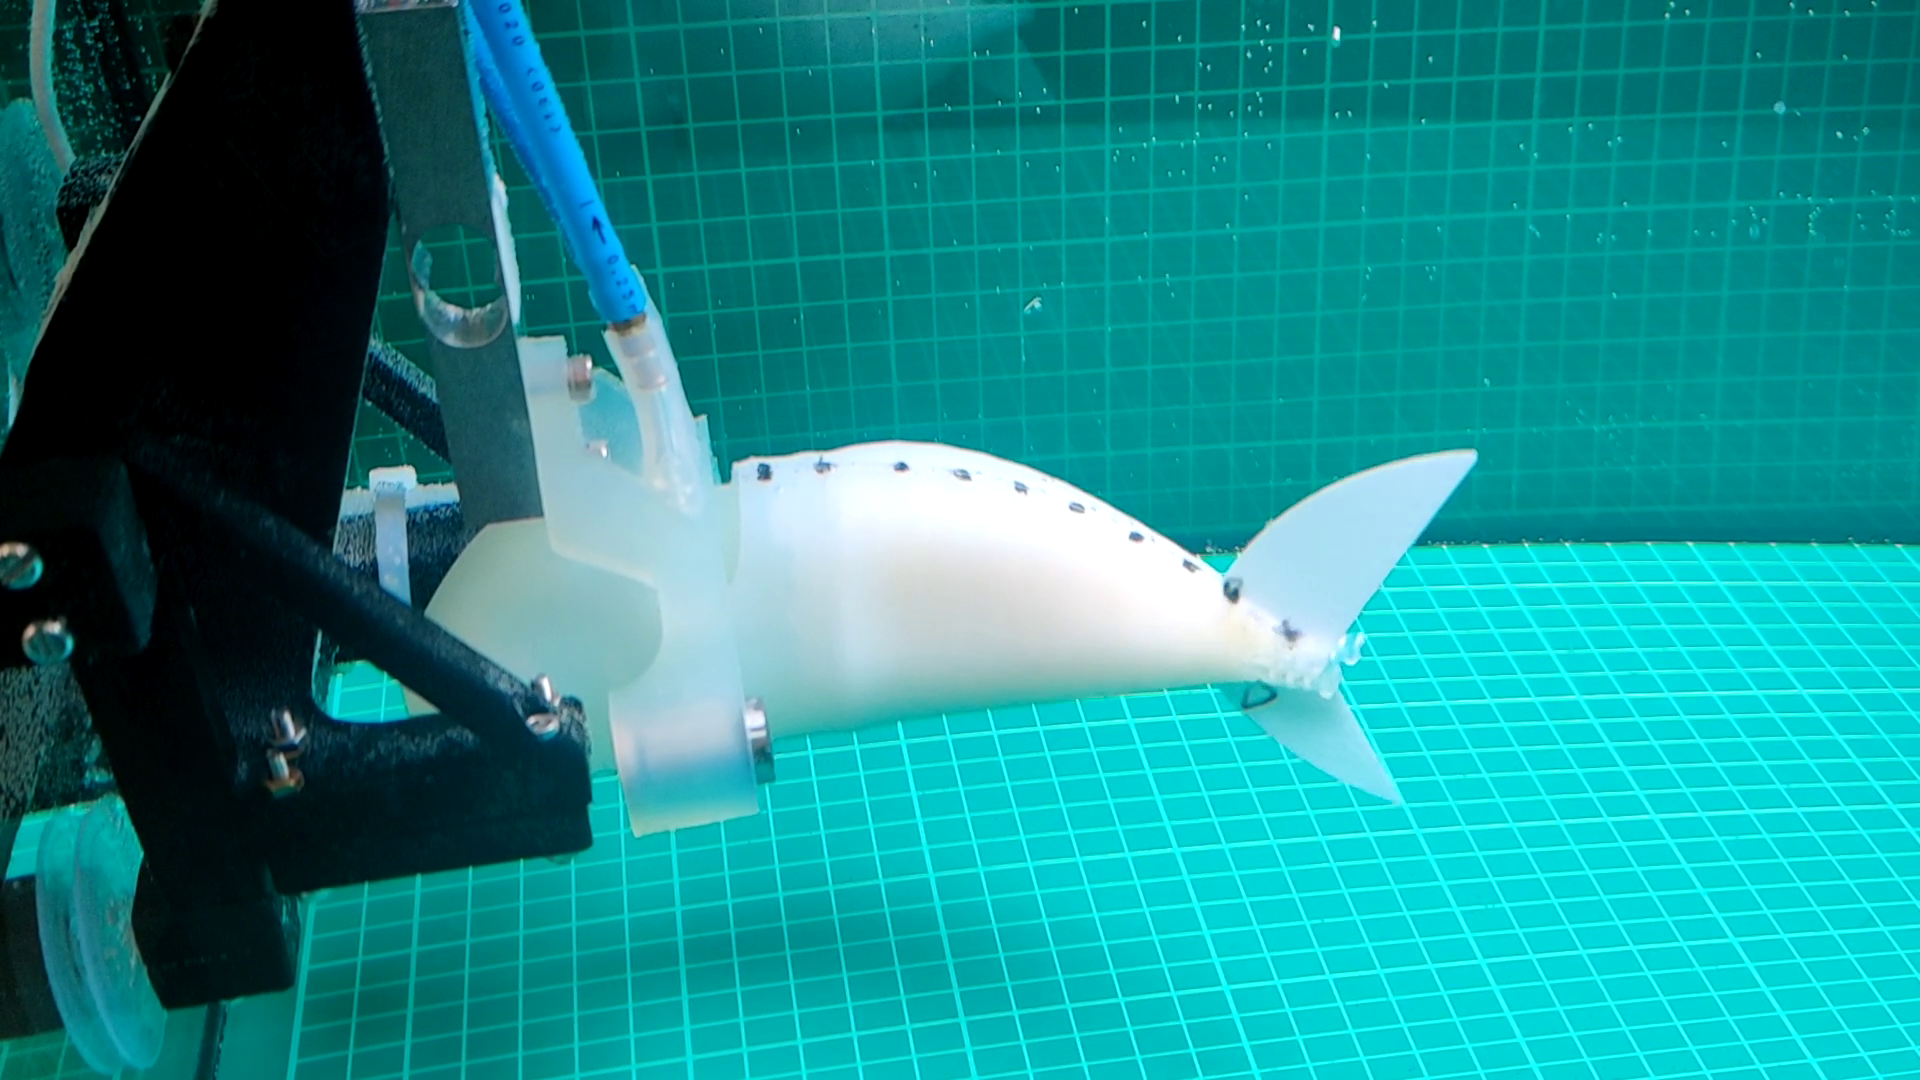
\includegraphics[width=0.9\columnwidth]{figures_appendix/thrust_jig.png}
    \caption{Test jig for measuring the thrust of the robotic fish. A 3D-printed fixture (black) connects the load cell (grey) to a fish adapter (opaque). The fish adapter is mounted within a casted soft robotic fish tail made of silicone elastomer. The fish tail has marker points along its back to enable motion tracking.}
    \label{fig:thrust_fixture}
\end{figure}
\fi

\iffalse
\subsection{Further Results for the Force Predictor}
In \Cref{fig:Bruce1}, we present generalization to different actuation pressures. In \Cref{fig:Bruce2} and \Cref{fig:Bruce3}, we present generalization to new trials of the same actuation signal. In \Cref{fig:Nemo1} and \Cref{fig:Nemo2}, we present generalization to unseen actuation frequencies.
%\Cref{tab:additional_trials} illustrates the training and tests sets used for additional trials.
\fi
\iffalse
\begin{table}[htb]
\caption{Additional combinations of training and test sets for the thrust predictor network.}
\centering
\begin{tabular}{|c|c|c|c|c|}
    \hline
    \textbf{Name} & \textbf{Mode} & \textbf{N.\ trials} & \textbf{Pressure} & \textbf{Frequency} \\
    \hline\hline
    \multirow{2}*{Nemo} & Training & 30 & 200,300 mbar & 1,2,3,4 Hz \\ \cline{2-5} & Validation & 10 & 200,300 mbar & 1 Hz \\
    \hline
    \multirow{2}*{Bruce} & Training & 32 & 500,750 mbar & 1,2,3,4 Hz \\ \cline{2-5} & Validation & 8 & 500,750 mbar & 1,2,3,4 Hz \\
    \hline
\end{tabular}
\label{tab:additional_trials}
\end{table}
\fi

\iffalse
\begin{figure}[htb]
    \centering
    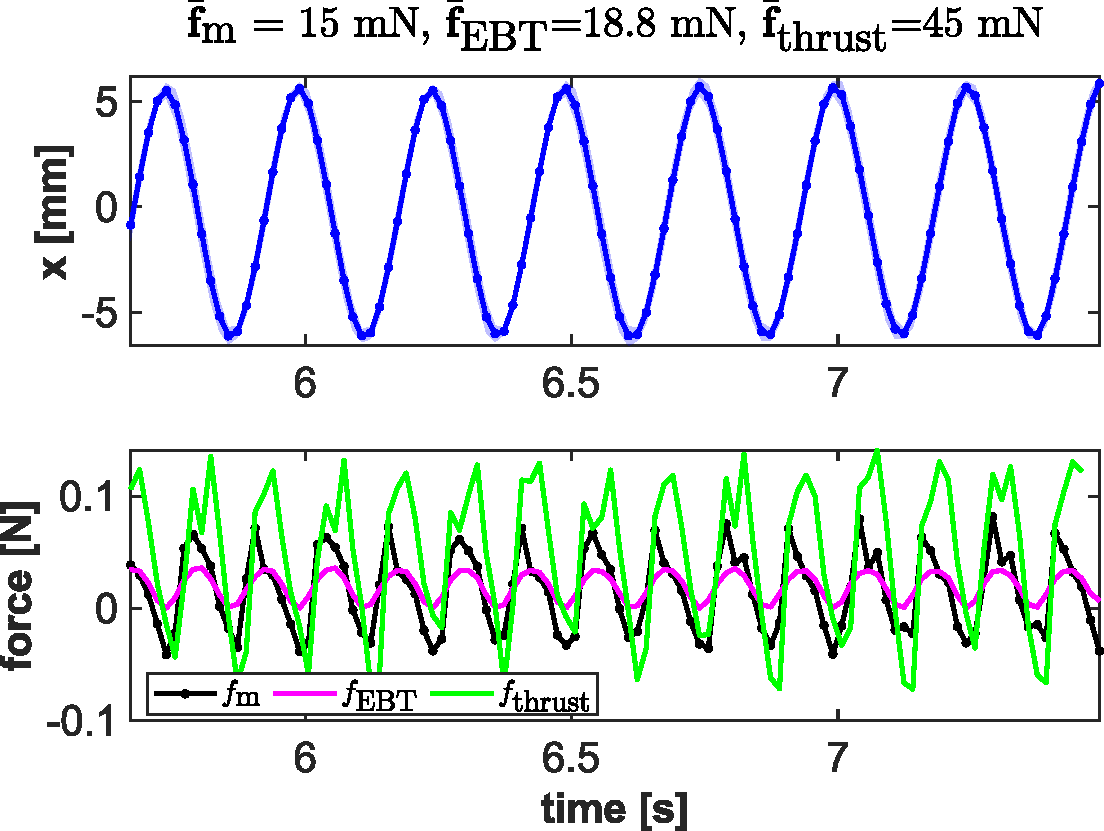
\includegraphics[width=0.8\columnwidth]{figures_appendix/error_analysis_500_mbar_4_Hz.pdf}
    \caption{Test set for \emph{Bruce} fish \SI{500}{mbar} at \SI{4}{Hz}. We attempt to generalize to lower actuation pressures having trained on higher actuation pressures. Generalization is poor, but frequency is correct. More data at different actuation pressures is likely needed for better generalization.}
    \label{fig:Bruce1}
\end{figure}
\begin{figure}[h]
    \centering
    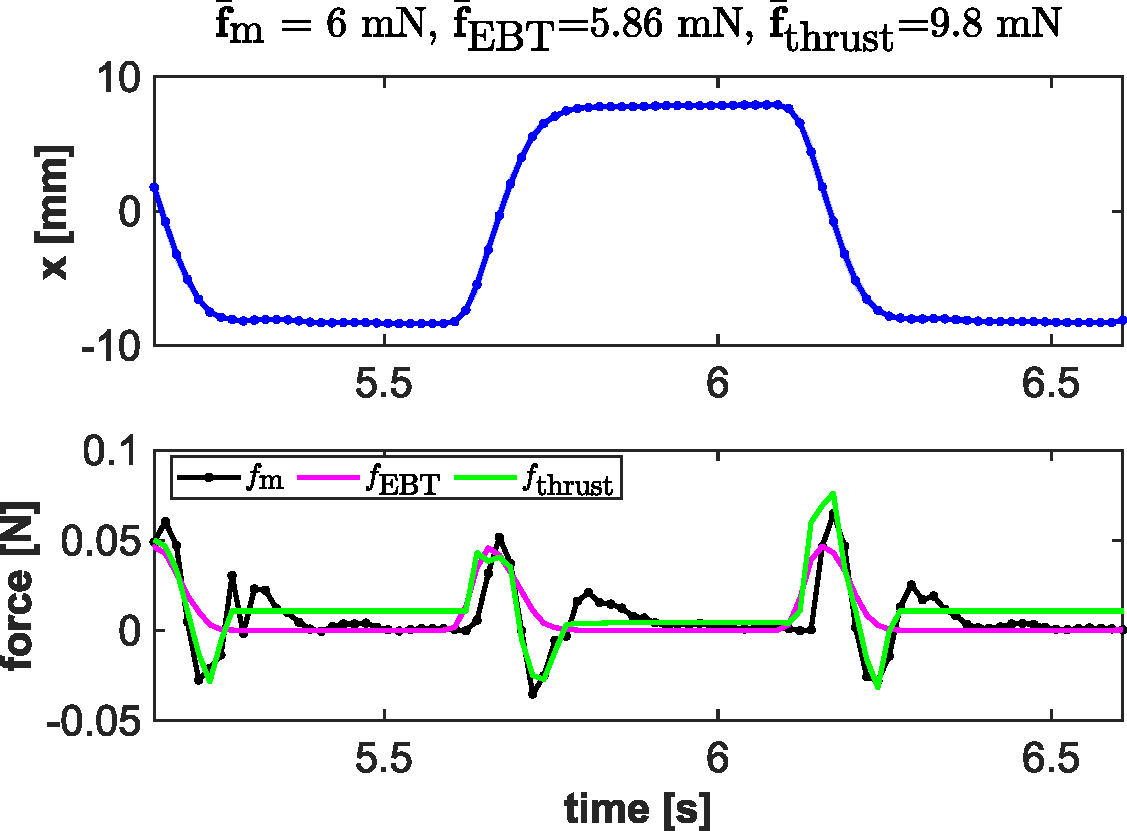
\includegraphics[width=0.8\columnwidth]{figures_appendix/error_analysis_500_mbar_1_Hz.pdf}
    \caption{Test set for \emph{Bruce} fish \SI{500}{mbar} at \SI{1}{Hz}. We predict an unseen trial having trained on data with the same actuation signal. Generalization is very good to unseen test cases.}
    \label{fig:Bruce2}
\end{figure}
\begin{figure}[h]
    \centering
    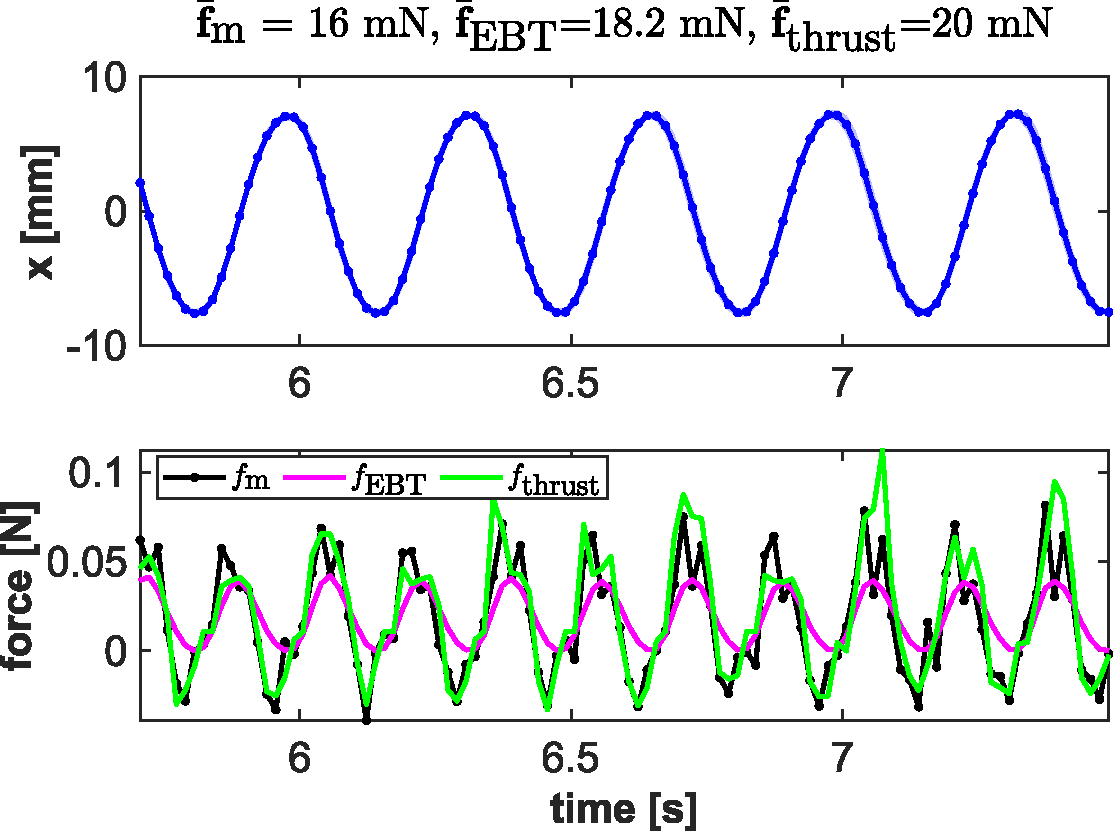
\includegraphics[width=0.8\columnwidth]{figures_appendix/error_analysis_500_mbar_3_Hz.pdf}
    \caption{Test set for \emph{Bruce} fish \SI{500}{mbar} at \SI{3}{Hz}. We predict an unseen trial having trained on data with the same actuation signal. Generalization is very good to unseen test cases.}
    \label{fig:Bruce3}
\end{figure}
\begin{figure}[h]
    \centering
    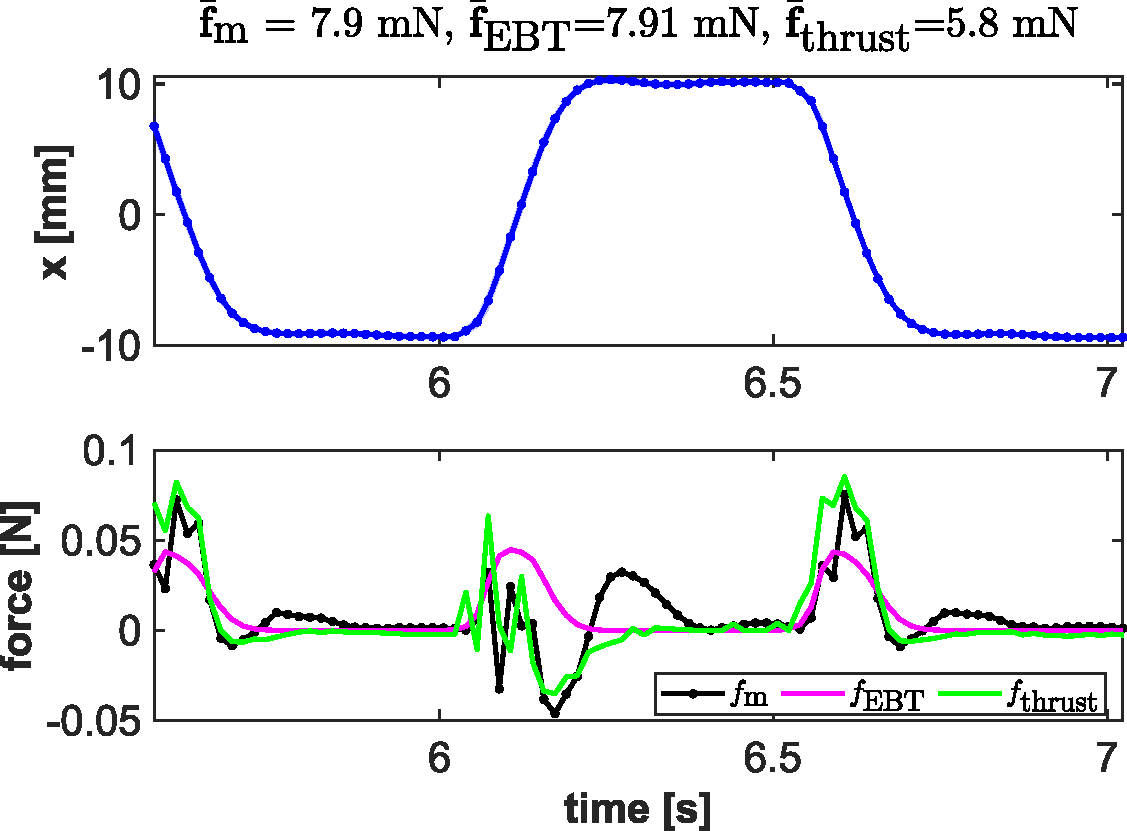
\includegraphics[width=0.8\columnwidth]{figures_appendix/error_analysis_200_mbar_1_Hz.pdf}
    \caption{Test set for \emph{Nemo} fish \SI{200}{mbar} at \SI{1}{Hz}. We use an unseen frequency as a test case. We observe good matching especially generalizing from higher to lower frequencies.}
    \label{fig:Nemo1}
\end{figure}
\begin{figure}[h]
    \centering
    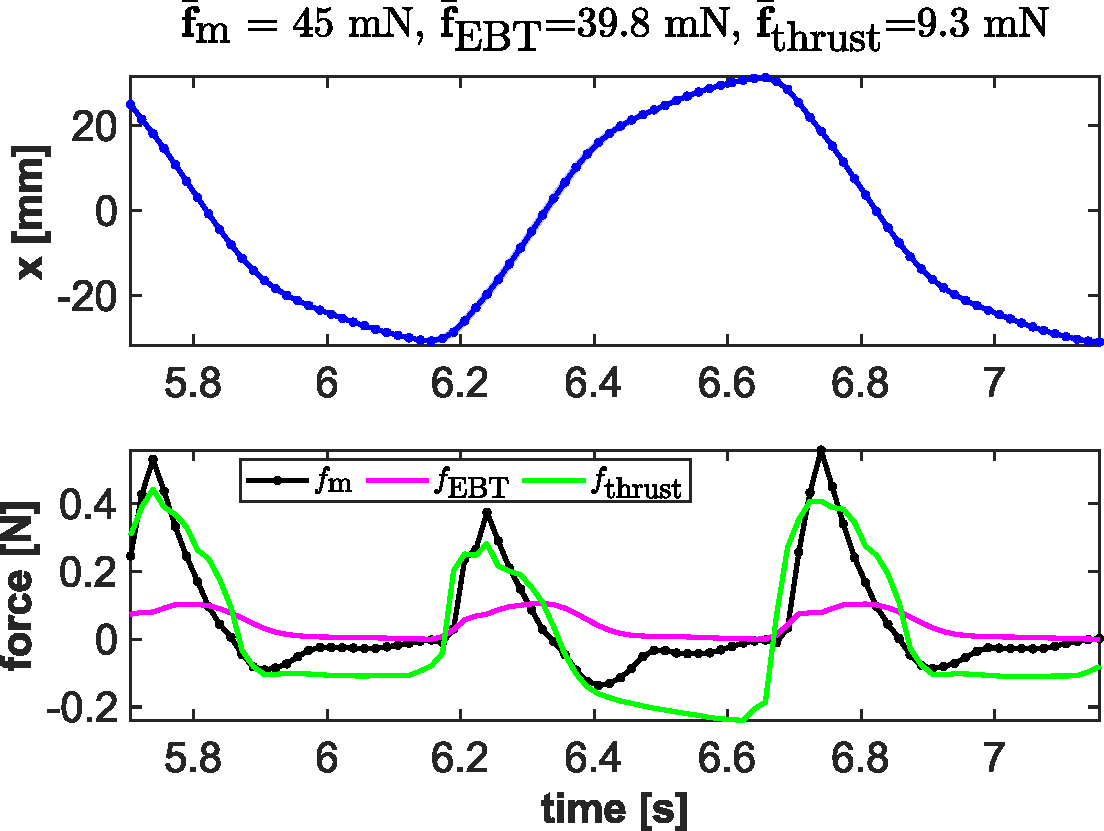
\includegraphics[width=0.8\columnwidth]{figures_appendix/error_analysis_300_mbar_1_Hz.pdf}
    \caption{Test set for \emph{Nemo} fish \SI{300}{mbar} at \SI{1}{Hz}. We use an unseen frequency as a test case. We observe good matching especially generalizing from higher to lower frequencies.}
    \label{fig:Nemo2}
\end{figure}
\fi